\documentclass[10pt, tikz]{standalone}


\begin{document}
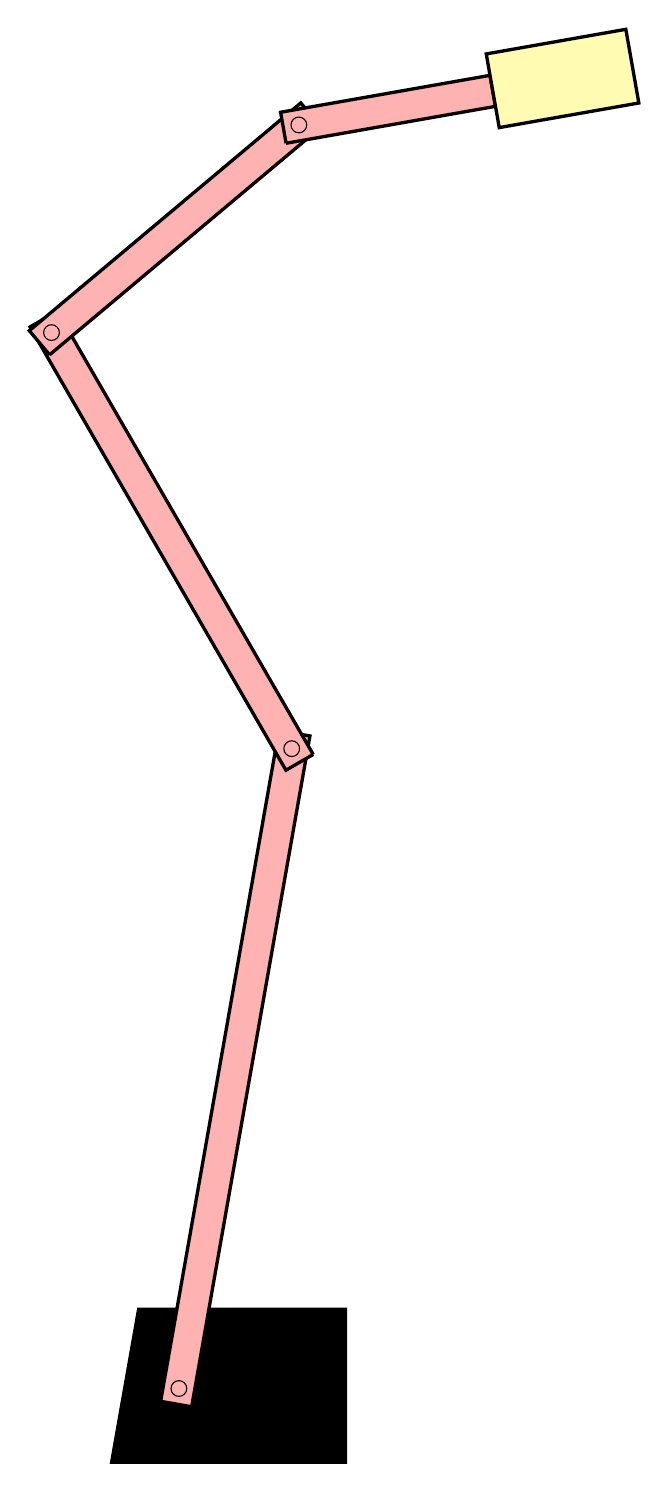
\begin{tikzpicture}[
scale=.1,
rod/.style={very thick, fill=red!30},
lamp/.style={very thick, fill=yellow!30},
bock/.style={fill},
]

\def\alp{80}
\def\bet{40}
\def\gam{-80}
\def\del{-30}

\def\b{4}			% Breite
\def\lA{86.5}		% Laenge 1
\def\lB{65}		% Laenge 2
\def\lC{45}		% Laenge 3
\def\lD{27}		% Laenge 4
% Lampe
\def\Ll{18}		% Laenge Lampe
\def\Lb{14}		% Breite Lampe 14 unten / 8 oben
\def\Lh{9.5}		% Hoehe Lampe


\path (0,0)coordinate(0);

\draw[bock] (0)++(\alp+90:\b/2)++(\alp:10)--++(-5,0)--++(\alp+180:20)--++(30,0)|-cycle;


\draw[rod] (0)++(\alp-90:\b/2)++(\alp-180:\b/2)--++(\alp:\lA)--++(\alp+90:\b)coordinate(1_)--++(\alp+180:\lA)--++(\alp-90:\b);

\pgfmathsetmacro{\be}{\alp+\bet}
\draw[rod] (1_)++(\alp-90:\b/2)++(\alp+180:\b/2)coordinate(1) ++(\be-90:\b/2)++(\be-180:\b/2)--++(\be:\lB)--++(\be+90:\b)coordinate(2_)--++(\be+180:\lB)--++(\be-90:\b);


\pgfmathsetmacro{\ga}{\alp+\bet+\gam}
\draw[rod] (2_)++(\be-90:\b/2)++(\be+180:\b/2)coordinate(2) ++(\ga-90:\b/2)++(\ga-180:\b/2)--++(\ga:\lC)--++(\ga+90:\b)coordinate(3_)--++(\ga+180:\lC)--++(\ga-90:\b);

\pgfmathsetmacro{\de}{\alp+\bet+\gam+\del}
\draw[rod] (3_)++(\ga-90:\b/2)++(\ga+180:\b/2)coordinate(3) ++(\de-90:\b/2)++(\de-180:\b/2)--++(\de:\lD)--++(\de+90:\b)coordinate(4_)--++(\de+180:\lD)--++(\de-90:\b);

\draw (0)circle(1);
\draw (1)circle(1);
\draw (2)circle(1);
\draw (3)circle(1);



\draw[lamp] (4_)++(\de-90:2)coordinate(4)--++(\de-90:\Lh/2)--++(\de:\Ll)--++(\de+90:\Lh)--++(\de-180:\Ll)--cycle;




\end{tikzpicture}
\end{document}